\documentclass[]{article}
\usepackage[T1]{fontenc}
\usepackage{lmodern}
\usepackage{amssymb,amsmath}
\usepackage{ifxetex,ifluatex}
\usepackage{fixltx2e} % provides \textsubscript
% use upquote if available, for straight quotes in verbatim environments
\IfFileExists{upquote.sty}{\usepackage{upquote}}{}
\ifnum 0\ifxetex 1\fi\ifluatex 1\fi=0 % if pdftex
  \usepackage[utf8]{inputenc}
\else % if luatex or xelatex
  \ifxetex
    \usepackage{mathspec}
    \usepackage{xltxtra,xunicode}
  \else
    \usepackage{fontspec}
  \fi
  \defaultfontfeatures{Mapping=tex-text,Scale=MatchLowercase}
  \newcommand{\euro}{€}
\fi
% use microtype if available
\IfFileExists{microtype.sty}{\usepackage{microtype}}{}
\usepackage[margin=1in]{geometry}
\usepackage{color}
\usepackage{fancyvrb}
\newcommand{\VerbBar}{|}
\newcommand{\VERB}{\Verb[commandchars=\\\{\}]}
\DefineVerbatimEnvironment{Highlighting}{Verbatim}{commandchars=\\\{\}}
% Add ',fontsize=\small' for more characters per line
\usepackage{framed}
\definecolor{shadecolor}{RGB}{248,248,248}
\newenvironment{Shaded}{\begin{snugshade}}{\end{snugshade}}
\newcommand{\KeywordTok}[1]{\textcolor[rgb]{0.13,0.29,0.53}{\textbf{{#1}}}}
\newcommand{\DataTypeTok}[1]{\textcolor[rgb]{0.13,0.29,0.53}{{#1}}}
\newcommand{\DecValTok}[1]{\textcolor[rgb]{0.00,0.00,0.81}{{#1}}}
\newcommand{\BaseNTok}[1]{\textcolor[rgb]{0.00,0.00,0.81}{{#1}}}
\newcommand{\FloatTok}[1]{\textcolor[rgb]{0.00,0.00,0.81}{{#1}}}
\newcommand{\CharTok}[1]{\textcolor[rgb]{0.31,0.60,0.02}{{#1}}}
\newcommand{\StringTok}[1]{\textcolor[rgb]{0.31,0.60,0.02}{{#1}}}
\newcommand{\CommentTok}[1]{\textcolor[rgb]{0.56,0.35,0.01}{\textit{{#1}}}}
\newcommand{\OtherTok}[1]{\textcolor[rgb]{0.56,0.35,0.01}{{#1}}}
\newcommand{\AlertTok}[1]{\textcolor[rgb]{0.94,0.16,0.16}{{#1}}}
\newcommand{\FunctionTok}[1]{\textcolor[rgb]{0.00,0.00,0.00}{{#1}}}
\newcommand{\RegionMarkerTok}[1]{{#1}}
\newcommand{\ErrorTok}[1]{\textbf{{#1}}}
\newcommand{\NormalTok}[1]{{#1}}
\usepackage{graphicx}
% Redefine \includegraphics so that, unless explicit options are
% given, the image width will not exceed the width of the page.
% Images get their normal width if they fit onto the page, but
% are scaled down if they would overflow the margins.
\makeatletter
\def\ScaleIfNeeded{%
  \ifdim\Gin@nat@width>\linewidth
    \linewidth
  \else
    \Gin@nat@width
  \fi
}
\makeatother
\let\Oldincludegraphics\includegraphics
{%
 \catcode`\@=11\relax%
 \gdef\includegraphics{\@ifnextchar[{\Oldincludegraphics}{\Oldincludegraphics[width=\ScaleIfNeeded]}}%
}%
\ifxetex
  \usepackage[setpagesize=false, % page size defined by xetex
              unicode=false, % unicode breaks when used with xetex
              xetex]{hyperref}
\else
  \usepackage[unicode=true]{hyperref}
\fi
\hypersetup{breaklinks=true,
            bookmarks=true,
            pdfauthor={},
            pdftitle={Regression Models Course Project Report},
            colorlinks=true,
            citecolor=blue,
            urlcolor=blue,
            linkcolor=magenta,
            pdfborder={0 0 0}}
\urlstyle{same}  % don't use monospace font for urls
\setlength{\parindent}{0pt}
\setlength{\parskip}{6pt plus 2pt minus 1pt}
\setlength{\emergencystretch}{3em}  % prevent overfull lines
\setcounter{secnumdepth}{0}

\title{Regression Models Course Project Report}
\author{}
\date{}

\begin{document}

\begin{center}
\huge Regression Models Course Project Report \\[0.2cm]
\end{center}
\normalsize


\section{Regression Models Course Project
Report}\label{regression-models-course-project-report}

\subsection{Martin Hediger}\label{martin-hediger}

\subsubsection{Executive Summary}\label{executive-summary}

This short report analyses if 1) automatic or manual transmission
results in larger miles-per-gallon (mpg) and 2) quantifies the effect of
manual or automatic transmission on mpg in the cars from the
\texttt{mtcars} dataset.\\Automatic transmission vehicles appear to be
less efficient than manual transmission vehicles (Fig. ``box-scat'' A).
A linear relationship between miles-per-gallon range and car weight for
both automatic and manual transmission vehicles is found (Fig.
``box-scat'' B).

\subsubsection{Exploratory Analysis}\label{exploratory-analysis}

As an initial test, dependence of \texttt{mpg} on \texttt{wt} is
analysed.\\\href{https://github.com/mzhKU/regmods_course_project/blob/master/box-scat.R}{\texttt{box-scat}}
A: Boxplot, B: Scatterplot of \texttt{mpg} against \texttt{wt}.

\begin{verbatim}
## Loading required package: grid
\end{verbatim}

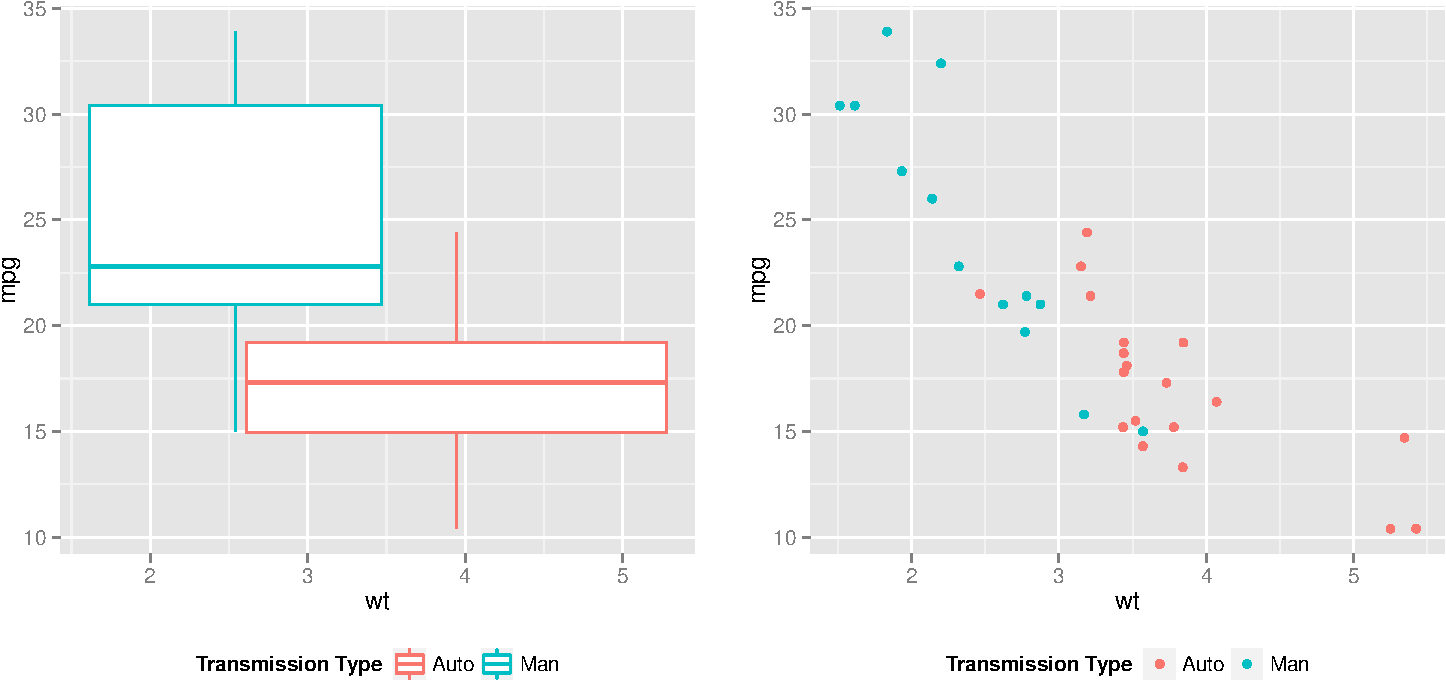
\includegraphics{./min_files/figure-latex/unnamed-chunk-1.pdf}

\href{https://github.com/mzhKU/regmods_course_project/blob/master/multiplot.R}{Source
code for the panel plot}.

According to the boxplot, automatic cars have lower MPG (and possibly
lower variance in the data). Importantly, the relationships appear
linear and no outliers which could affect correlation values are
identified. The only aspect which is slightly problematic is the limited
dataset size (n=32).\\It is noted that apparently most cars with
automatic transmission also are heavier which possibly confounds the
observation, this would be subject to further research.

\subsubsection{Results}\label{results}

\textbf{Question 1: Which transmission type has higher MPG?}\\Based on
the exploratory analysis above, it is found that on average the
difference between MPG(auto) and MPG(man) is around 7.2449
miles-per-gallon
(=\texttt{mean(mtcars{[}mtcars\$am==1, "mpg"{]}) - mean(mtcars{[}mtcars\$am==0, "mpg"{]})}).

\textbf{Question 2: Quantification of MPG-difference between
transmission types}\\MODEL 1\\First, the full model is assessed,
i.e.~dependence of \texttt{mpg} on all other variables:

\begin{Shaded}
\begin{Highlighting}[]
\NormalTok{fit_full <-}\StringTok{ }\KeywordTok{lm}\NormalTok{(mpg ~ . +}\StringTok{ }\KeywordTok{factor}\NormalTok{(am), }\DataTypeTok{data=}\NormalTok{mtcars)}
\KeywordTok{summary}\NormalTok{(fit_full)$coefficients}
\end{Highlighting}
\end{Shaded}

\begin{verbatim}
##             Estimate Std. Error t value Pr(>|t|)
## (Intercept) 12.30337   18.71788  0.6573  0.51812
## cyl         -0.11144    1.04502 -0.1066  0.91609
## disp         0.01334    0.01786  0.7468  0.46349
## hp          -0.02148    0.02177 -0.9868  0.33496
## drat         0.78711    1.63537  0.4813  0.63528
## wt          -3.71530    1.89441 -1.9612  0.06325
## qsec         0.82104    0.73084  1.1234  0.27394
## vs           0.31776    2.10451  0.1510  0.88142
## am           2.52023    2.05665  1.2254  0.23399
## gear         0.65541    1.49326  0.4389  0.66521
## carb        -0.19942    0.82875 -0.2406  0.81218
\end{verbatim}

\end{document}
